\chapter{힘, 쿼크, 그리고 최초의 강입자 다중항}

\section{입자, 장, 그리고 빠진 세 번째 요소}

파동은 장의 배열이므로, 이 논의에서는 두 설명이 밀접하게 관련되어 있다. 양자역학에 따르면 그런 파동의 에너지는 불연속적인 불가분 단위로 주어진다. 이 단위가 양자이며, 장의 양자가 바로 입자라고 부르는 것이다. 이 관계를 바탕으로 우리는 이미 파동방정식, 작용 원리, 그리고 입자가 지니는 에너지, 운동량, 스핀, 보손--페르미온 구분 같은 전반적인 성질을 논의했다. 페르미온은 같은 상태를 점유하는 것을 꺼리는 반면, 보손은 한 상태에 모여 응축할 수 있다.

양자 라그랑지안에는 상호작용도 기록된다. 장의 곱은 입자가 들어오고 나가는 꼭짓점을 나타낸다. 예를 들어 장의 네 제곱을 포함하는 항은 네 다리 상호작용 꼭짓점을 나타낸다. 이처럼 작용 원리는 가능한 입자 과정의 목록을 간결하게 정리한다.

다음 과제는 입자들의 이름을 붙이고------각 입자에 고유한 성격, 즉 성질과 상호작용, 일상적인 물리에서의 역할을 부여하는 것이다. 하지만 그 목록을 만들기 전에 개념적 삼각형의 한 변이 아직 빠져 있다.
\begin{itemize}
\item 입자,
\item 그 입자들이 양자인 장,
\item 바로 그 양자들이 관여하는 교환 과정과 관련된 힘.
\end{itemize}

\emph{기본}이라는 말은 잠정적으로만 써야 한다. 복합 입자와 구별되는 기본 입자를 정의하려 하면, 그럴듯한 정의는 결국 모호한 사례와 마주치게 된다. 이 문제는 뒤에서 다시 다루겠다. 지금은 기본 장이 존재한다고 가정하고, 그 양자를 기본 입자라고 부르자. 전기장이 전기력을 일으키고 중력장이 중력을 일으킨다면, 전자장도 힘에 관여해야 한다. 힘을 장으로 설명하는 동시에 입자로도 설명할 수 있어야 이 삼각형이 닫힌다.

그러므로 힘의 논리를 두 번 유도하겠다. 먼저 고전 장 에너지를 이용한 다음, 장을 양자로 분해했을 때 같은 상호작용이 어떻게 나타나는지 살펴본다. 이 두 설명을 잇는 가교가 확실해진 뒤에야 입자 목록을 시작하겠다.

\section{고전 전기역학에서 장 에너지로부터 힘을 구하기}

공간에 두 전하를 놓아 보자. 두 전하 사이의 힘을 구하는 한 방법은 역제곱 법칙을 인용하는 것이다. 더 많은 것을 보여 주는 방법은 전하가 공간에 어떤 영향을 주는지 묻는 것이다. 전하는 전기장을 만들고, 그 장은 에너지를 저장한다.

각 전하와 그 전하가 만드는 장의 공간적 형태를 분리해 두는 것이 편리하다.
\begin{equation}
\mathbf E_i=q_i\widehat{\mathbf E}_i,
\end{equation}
모자 표기를 유지하는지는 결과에 영향을 주지 않는다. 두 전하가 모두 있을 때 선형성에 따라
\begin{equation}
\mathbf{E}=\mathbf{E}_1+\mathbf{E}_2.
\end{equation}
단위계 선택에 따른 차이를 제외하면 정전기장의 에너지는 다음 형태를 갖는다.
\begin{equation}
U_{\text{field}}\propto\int d^3x\,\mathbf{E}^2.
\end{equation}
두 장의 합을 대입하면
\begin{align}
U_{\text{field}}
&\propto\int d^3x\,(\mathbf{E}_1+\mathbf{E}_2)^2 \\
&\propto\int d^3x\,\bigl(\mathbf{E}_1^2+\mathbf{E}_2^2
  +2\mathbf{E}_1\!\cdot\!\mathbf{E}_2\bigr).
\end{align}

앞의 두 항은 자기 에너지다. 어느 한 전하를 옮기면 그 전하의 장도 함께 이동하므로, 해당 적분값은 변하지 않는다. 이 에너지는 \(E=mc^2\)를 통해 고립된 대전 입자의 측정 질량에 기여한다. 이 자기 에너지가 측정 질량에 어떻게 반영되는지는 나중에 다룰 재규격화의 주제다. 위치에 무관한 이 에너지는 어느 것도 두 입자 사이의 힘에 기여하지 않는다.

교차항은 다르다. 이 항은 어느 한 입자에만 속하지 않으며 두 장이 모두 있을 때에만 존재한다. 두 전하를 아주 멀리 떨어뜨리면 유의미한 장 영역은 거의 겹치지 않는다. 전하가 가까워지면 겹치는 정도가 달라진다. 따라서 배열에 따라 달라지는 상호작용 에너지는 다음에 비례한다.
\begin{equation}
U_{\text{int}}(r)\propto q_1q_2\int d^3x\,
\widehat{\mathbf E}_1\!\cdot\!\widehat{\mathbf E}_2.
\end{equation}
두 점전하 사이의 거리가 \(r\)일 때 적분을 계산하면 익숙한 의존성이 나온다.
\begin{equation}
U_{\text{int}}(r)\propto\frac{q_1q_2}{r}.
\end{equation}
방사 방향 힘은 이 에너지의 음의 기울기다.
\begin{equation}
\mathbf F_{12}=-\boldsymbol\nabla_{\mathbf r}U_{\text{int}},
\qquad
|\mathbf F_{12}|\propto\frac{|q_1q_2|}{r^2}.
\end{equation}
\editorialnote{강의에서 말로 설명한 논증은 퍼텐셜을 따로 거치지 않고 교차항을 역제곱 쿨롱 힘과 연결한다. 여기서는 그 기울기가 명시된 \(1/r^2\) 힘을 주도록 표준적인 중간 단계인 \(U_{\mathrm{int}}\propto1/r\)를 적어 둔다.}

힘의 법칙은 이제 상대적 위치에 따라 달라지는 장 에너지 부분의 미분으로 표현된다. 두 물체가 멀리 떨어져 있으면 사실상 서로 독립적이다. 두 물체를 가까이 가져오면 그 사이의 장이 재배열되고, 그 결과 에너지가 변한다. 이것이 상호작용이다.

하지만 장을 양자로 분해할 수 있다면, 이것으로 이야기가 끝날 수는 없다. 같은 힘을 입자의 언어로도 설명할 수 있어야 한다.

\section{분자 교환: 양성자 두 개와 전자 한 개}

전기역학으로 돌아가기 전에 교환을 더 쉽게 그려 볼 수 있는 계, 즉 양성자 두 개와 전자 한 개로 이루어진 계를 살펴보자. 교환은 분자력의 여러 기원 가운데 하나일 뿐이지만, 이 예에서는 교환과 에너지, 힘의 관계를 분명히 볼 수 있다. 이 예는 양자전기역학을 대신하려는 것이 아니다.

양성자 하나만 있고 다른 양성자가 무한히 멀리 떨어져 있다면, 전자는 첫 번째 양성자에 중심을 둔 수소형 바닥 상태를 차지할 수 있다. 그 파동함수는 해당 힘의 중심 부근에 국소화되어 있다.

\begin{figure}[h]
\centering
\includegraphics[width=0.72\textwidth]{lecture_01_figure_02.png}

\medskip

\begin{tikzpicture}[scale=0.95]
\draw (-0.2,0) -- (6.4,0);
\fill (1.3,0) circle (2pt);
\draw[smooth] plot coordinates {(0.1,0.15) (0.8,1.15) (1.5,1.75) (2.2,1.1) (3.0,0.35) (3.8,0.12)};
\node at (1.3,-0.35) {$p$};
\node at (2.7,1.55) {$\psi_1(x)$};
\end{tikzpicture}
\caption{한 양성자 부근에 국소화된 수소형 바닥 상태 파동함수.}
\lectureframe{00:14:32}
\end{figure}
\editorialnote{다시 그린 그림의 \(\psi_1(x)\) 표기는 00:14:30에서 설명한 국소화된 형태를 가리킨다. 읽을 수 있는 판서의 표기를 옮긴 것은 아니다.--00:14:32}

이제 두 번째 양성자를 유한하지만 큰 거리에 놓자. 대칭성에 따라 같은 한 중심 에너지를 갖는 두 번째 국소화 상태가 생기며, 이번에는 오른쪽 양성자를 중심으로 한다.

\begin{figure}[h]
\centering
\includegraphics[width=0.78\textwidth]{lecture_01_figure_03.png}

\medskip

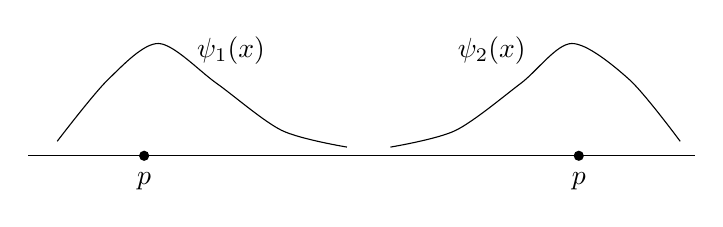
\begin{tikzpicture}[scale=0.92]
\draw (-0.2,0) -- (9.0,0);
\fill (1.4,0) circle (2pt);
\fill (7.4,0) circle (2pt);
\draw[smooth] plot coordinates {(0.2,0.2) (0.9,1.05) (1.6,1.55) (2.4,1.0) (3.3,0.35) (4.2,0.12)};
\draw[smooth] plot coordinates {(4.8,0.12) (5.7,0.35) (6.6,1.0) (7.3,1.55) (8.1,1.05) (8.8,0.2)};
\node at (1.4,-0.35) {$p$};
\node at (7.4,-0.35) {$p$};
\node at (2.6,1.45) {$\psi_1(x)$};
\node at (6.2,1.45) {$\psi_2(x)$};
\end{tikzpicture}
\caption{터널링을 허용한 뒤 평형 중첩 상태를 만드는 데 사용되는 두 국소화 파동함수.}
\lectureframe{00:17:54}
\end{figure}
\editorialnote{표기 \(\psi_1(x)\)와 \(\psi_2(x)\)는 00:17:41에서 논의한 두 형태를 가리킨다. 기호는 읽기 쉽도록 덧붙인 개략적인 표기다.--00:17:56}

거리가 무한대일 때 두 상태는 축퇴되어 있다. 전자를 왼쪽이나 오른쪽에 국소화해도 에너지는 같다. 거리가 유한하면 새로운 과정이 가능해진다. 전자는 고전적으로 금지된 영역을 지나 한 중심에서 다른 중심으로 터널링할 수 있다. 장벽을 통과하는 궤적을 관찰하려 하면 상태를 교란하게 된다. ``도약''은 고전적 경로를 촬영한 영상이 아니라 양자적 시간 전개의 설명이다.

평형 상태에서 전자는 두 양성자 가운데 어느 쪽 부근에서 발견될 확률도 같다. 따라서 정규화 계수는 \(1/\sqrt2\)이며, 더 낮은 평형 상태는 근사적으로 다음과 같다.
\begin{equation}
\psi_+(x)\approx \frac{\psi_1(x)+\psi_2(x)}{\sqrt2}.
\end{equation}

근사 기호가 중요하다. 실제 두 중심 파동함수는 변형되지 않은 두 수소형 궤도함수의 합과 정확히 같지 않으며, 겹침 영역에서 모양이 조정된다. 여기서 필요한 요점은 대칭 평형 상태의 에너지가 고립된 한 중심의 에너지보다 낮다는 것이다. 해밀토니안으로 표현하면 왼쪽과 오른쪽 배열은 비대각 행렬 원소로 결합되어 있다. 전자가 두 상태의 결맞은 중첩을 차지하도록 허용하면 에너지가 낮아진다.

\section{낮아진 에너지에서 유효 힘으로}

양성자 사이의 거리가 클 때 전자로 인해 생기는 기여분 \(E_e(r)\)는 분리된 원자의 값에 가까워진다. 거리가 줄면 터널링과 중첩으로 이 값이 낮아진다. 두 양성자--와 전자 하나로 이루어진 계의 전체 퍼텐셜에는 양성자 사이의 직접적인 반발도 포함되어야 한다.
\begin{equation}
V_{\mathrm{tot}}(r)=V_{pp}(r)+E_e(r).
\end{equation}

이로써 분자 예시는 장 에너지 논증과 다시 연결된다. 파동함수 그림과 \(E_e(r)\)의 정성적 곡선은 같은 계산을 두 가지 방식으로 보여 준다. 평형은 두 기여분의 합인 \(V_{\mathrm{tot}}(r)\)로 결정된다.

\begin{figure}[h]
\centering
\includegraphics[width=0.78\textwidth]{lecture_01_figure_04.png}

\medskip

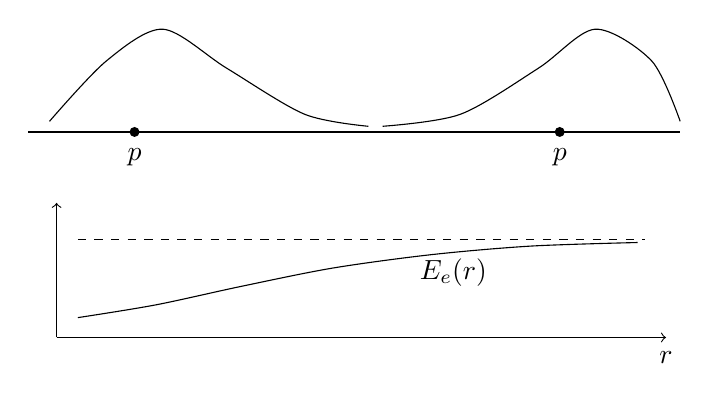
\begin{tikzpicture}[scale=0.9]
\draw (-0.2,3.0) -- (9.0,3.0);
\fill (1.3,3.0) circle (2pt);
\fill (7.3,3.0) circle (2pt);
\draw[smooth] plot coordinates {(0.1,3.15) (0.9,4.0) (1.7,4.45) (2.6,3.9) (3.7,3.25) (4.6,3.08)};
\draw[smooth] plot coordinates {(4.8,3.08) (5.9,3.25) (7.0,3.9) (7.8,4.45) (8.6,4.0) (9.0,3.15)};
\node at (1.3,2.65) {$p$};
\node at (7.3,2.65) {$p$};

\draw[->] (0.2,0.1) -- (0.2,2.0);
\draw[->] (0.2,0.1) -- (8.8,0.1);
\draw[dashed] (0.5,1.48) -- (8.5,1.48);
\draw[smooth] plot coordinates {(0.5,0.38) (1.6,0.56) (2.8,0.82) (4.1,1.08) (5.5,1.27) (6.9,1.39) (8.4,1.44)};
\node at (5.8,1.02) {$E_e(r)$};
\node at (8.8,-0.18) {$r$};
\end{tikzpicture}
\caption{위쪽은 파동함수의 겹침, 아래쪽은 전자로 인해 생기는 에너지를 나타낸다. \(r\)가 증가하면 분리된 원자의 점근값에 가까워지며, 양성자 전체 퍼텐셜에는 양성자 사이의 쿨롱 반발도 포함해야 한다.}
\lectureframe{00:20:28}
\end{figure}
\editorialnote{표기 \(E_e(r)\)와 \(r\)는 00:19:12에서 논의한 에너지 곡선과 거리를 가리킨다. 남아 있는 판서 화면으로는 축 표기를 읽을 수 없다.--00:20:38}

두 힘은 각각 에너지의 기울기로부터 나온다.
\begin{equation}
F_{e}(r)=-\frac{dE_e}{dr},
\qquad
F_{\mathrm{tot}}(r)=-\frac{dV_{\mathrm{tot}}}{dr}.
\end{equation}
따라서 계는 전체 에너지가 낮아지는 방향으로 힘을 받는다. 양성자들이 가까워질수록 \(E_e(r)\)가 감소하는 범위에서는 교환이 인력 성분을 제공한다. 결합된 거리가 존재하는지는 이 인력 성분과 \(V_{pp}(r)\) 사이의 경쟁에 달려 있다. 이것이 공유 결합의 기본 메커니즘이다. 전자가 공유 상태에 있는 까닭은 그 상태의 에너지가 더 낮기 때문이다.

고전적 계산에서는 전기장이 겹치면서 에너지가 달라진다. 여기서는 두 힘의 중심이 더 낮은 양자 상태를 가능하게 한다. 두 메커니즘 모두 평형 에너지가 배열에 따라 달라지기 때문에 힘을 만들어 낸다.

교환을 나타내는 세계선 그림으로 이 설명을 요약할 수 있다. 이를 관측된 궤적으로 읽어서는 안 된다. 전자가 어느 쪽 양성자와 결부될 수 있는지를 나타내는 진폭을 표현한 그림이다.

\begin{figure}[h]
\centering
\begin{tikzpicture}[scale=1.0]
\draw (0,0) -- (0,4.4);
\draw (4.8,0) -- (4.8,4.4);
\draw (0,0.9) .. controls (1.6,1.7) and (3.2,1.7) .. (4.8,2.5);
\draw (4.8,2.9) .. controls (3.2,2.1) and (1.6,2.1) .. (0,3.9);
\node at (0,-0.35) {$p$};
\node at (4.8,-0.35) {$p$};
\node at (2.35,1.55) {$e^-$};
\node at (2.35,2.55) {$e^-$};
\end{tikzpicture}
\caption{두 양성자 세계선 사이의 전자 교환. 관찰된 경로가 아니라 양자 진폭을 나타내는 개략도다.}
\end{figure}

\begin{classroomqa}
\audiencequestion{전자가 양성자 전하를 가리거나 줄여서 인력을 간단히 설명할 수 있나요?\lecturetimestamp{00:23:26}}
\lecturerresponse{아니요. 이 효과를 전하가 줄어드는 그림으로 설명하는 것은 적절하지 않습니다. 핵심은 두 국소화 파동함수를 더해 얻는 상태의 에너지가 각 국소화 상태의 에너지보다 조금 낮다는 점입니다.}
\end{classroomqa}

\begin{classroomqa}
\audiencequestion{파인먼이 ``빛은 빛을 좋아한다''고 한 말이 이런 뜻인가요?\lecturetimestamp{00:23:51}}
\lecturerresponse{아니요. 그 표현은 보손 통계와 관련이 있을 가능성이 큽니다. 광자는 같은 상태를 선호하는 반면 전자는 배타 원리를 따릅니다. 여기서 다루는 분자 효과는 두 중심 사이의 터널링입니다.}
\end{classroomqa}

두 양성자는 여전히 정전기적으로 서로 밀어낸다. 교환의 작용 범위는 쿨롱 상호작용보다 짧으므로, 어느 한 기여분만이 아니라 전체 퍼텐셜을 고려해야 한다. 적절한 거리에서는 분자 이온 \(\mathrm H_2^+\)이 그래도 결합 상태를 이룬다. 중성인 두 전자 계에서는 장거리 전하 반발이 없으므로 공유 결합이 더 익숙한 현상이다.

\begin{classroomqa}
\audiencequestion{양성자 사이에 전자를 두면 주로 정전기적 반발이 줄어드나요?\lecturetimestamp{00:24:33}}
\lecturerresponse{반발이 조금 줄기는 하지만, 그것이 주된 효과는 아닙니다. 전자 교환은 쿨롱 반발보다 작용 범위가 짧은 힘입니다. 장거리 정전기력이 원자 사이에 작용하지 않으면서도 터널링이 인력을 만드는 중성 두 전자 계에서 그 효과가 가장 뚜렷하게 나타납니다.}
\end{classroomqa}

\begin{classroomqa}
\audiencequestion{전자 하나만 가진 양전하 분자 이온 \(\mathrm H_2^+\)은 실제로 결합 상태인가요?\lecturetimestamp{00:26:06}}
\lecturerresponse{네. 충분히 가까운 거리에서는 교환 인력이 양성자--양성자 사이의 쿨롱 반발을 이길 만큼 강해집니다.}
\end{classroomqa}

\begin{classroomqa}
\audiencequestion{두 중심 배열이 세 번째 힘을 만들어 내나요?\lecturetimestamp{00:26:24}}
\lecturerresponse{새로운 기본 힘이 도입되는 것은 아닙니다. 두 양성자의 결합 퍼텐셜 안에서 Schr\"odinger 방정식을 풀면 한 중심 문제와 다른 평형 에너지가 나온다. 달라진 에너지를 미분한 값이 유효 힘이다.}
\end{classroomqa}

\begin{classroomqa}
\audiencequestion{에너지가 낮아지는 것이 양자 얽힘의 한 예인가요?\lecturetimestamp{00:27:06}}
\lecturerresponse{통상적인 두 입자 의미의 얽힘은 아닙니다. 전자 하나만 있으면 됩니다. 여기서 중요한 수학적 특징은 왼쪽 상태와 오른쪽 상태를 결합하는 비대각 해밀토니안 행렬 원소입니다.}
\end{classroomqa}

\begin{classroomqa}
\audiencequestion{온도가 높아지면 교환은 어떻게 되나요?\lecturetimestamp{00:27:37}}
\lecturerresponse{극한적인 고온에서는 전자가 이온화되어 분자와 더는 결부되지 않습니다. 더 낮은 들뜸 에너지에서는 전자가 더 큰 궤도에 있을 수 있으며, 이로 인해 겹침 정도와 힘이 달라집니다. 이는 상태에 따라 달라지는 보정이지, 새로운 일반적 메커니즘은 아닙니다.}
\end{classroomqa}

\section{광자 교환과 표의 첫 항목들}

쿨롱 힘도 같은 교환의 언어로 설명할 수 있을까? 대전 입자는 전자기장과 상호작용하고, 그 장의 양자는 광자다. 고전적으로는 전하 주변의 전기장을 구한다. 양자장론에서는 그 상호작용을 광자의 방출과 흡수로 분해해 기술한다.

실제 대전 입자는 단순히 맨전하만으로 이루어지지 않는다. 그 상태는 맨전자 성분, 광자 하나를 동반한 전자, 광자 둘을 동반한 전자 등을 포함하는 양자 중첩이다. 의도적으로 개략적인 표기법으로 쓰면 다음과 같다.
\begin{equation}
\begin{aligned}
\ket{e_{\mathrm{phys}}}
={}&a_0\ket e
+a_1\ket{e+\text{one photon}}
\\
&+a_2\ket{e+\text{two photons}}+\cdots .
\end{aligned}
\end{equation}
이 표기는 광자 수 성분의 계층만 나타낼 뿐, 광자 운동량을 지정하거나 상호작용하는 대전 상태를 완전히 구성하려는 것은 아니다.
주변 광자는 자유 복사로 빠져나가는 대신 방출되었다가 다시 흡수된다. 그 효과는 측정할 수 있지만 자유롭게 전파하는 광자와 같은 방식으로 검출되지는 않는다. 가까이에 두 번째 전하를 놓으면 한 전하가 방출한 광자를 다른 전하가 흡수할 수 있다. 그러면 두 드레싱된 상태의 에너지는 두 고립된 상태 에너지를 단순히 더한 값과 달라진다.

강의실에서 든 비유는 각자 공을 다루는 저글링하는 사람 둘이다. 두 사람이 멀리 떨어져 있으면 각자 독립적으로 저글링한다. 서로 가까이 오면 한 사람이 다른 사람이 던진 공을 받을 수 있다. 파인먼 도표 언어로 말하면 그 공통 대상은 교환된 광자다. 이 비유는 미시적인 궤적을 뜻하지 않지만, 가까이 있을 때 새로운 과정이 가능해지는 이유를 잘 보여 준다.

이제 쿨롱 법칙을 외우는 데 그치지 않는 두 가지 설명을 얻었다. 고전 장 이론에서는 장들을 더한 뒤 그 결과를 제곱한다. 양자장론에서는 양자가 교환되는 진폭들을 합산한다. 이런 의미에서 입자, 장, 힘은 일대일대일 대응을 이룬다. 전자는 분자 교환을 매개하고, 광자는 전자기 교환을 매개한다. 적절한 상황에서는 교환될 수 있는 입자라면 어느 것이든 고유한 유효 힘 성분에 기여할 수 있다. 따라서 자연에는 네 가지 기본 상호작용이 있다는 익숙한 진술은 더 큰 수준에서 분류한 것이다. 교환의 언어로 보면 교환 가능한 각 종이 그 자체의 유효 힘 성분을 만들어 낼 수 있다.

이제 입자의 이름을 붙이고, 성질을 나열하며, 어떤 과정에 참여할 수 있는지 설명할 차례다. 표준모형 전체를 한 번에 쓰면 긴 암기 시험이 될 뿐이므로, 서로 단순한 관계를 이루는 작은 입자군으로 나누어 각 군이 어떤 일을 할 수 있는지 알아보겠다.

전체 목록은 다소 복잡하다. 왜 바로 이 입자들이 존재하고 상상할 수 있는 다른 입자들은 존재하지 않는지 우리는 이해하지 못하기 때문이다. 수학적 일관성은 몇 가지 관계를 제약한다. 어떤 패턴의 구성원들이 여럿 존재하면, 그 패턴을 완성하기 위해 다른 구성원이 요구될 수도 있다. 이런 관계 덕분에 독립적으로 알아야 할 사실의 수는 줄지만, 그 감소 폭은 크지 않다. 많은 입자 종류와 많은 매개변수가 여전히 설명되지 않았다. 뒤이은 실험이 무엇을 발견하려 하는지 이해하려면 이 미완의 구조를 파악해야 한다.

\begin{figure}[h]
\centering
\includegraphics[width=0.7\textwidth]{lecture_01_figure_05.png}
\caption{입자 표의 첫 항목은 \(\gamma\)로 광자를, 벡터 퍼텐셜 \(A\)로 그 장을 나타낸다.}
\lectureframe{00:39:11}
\end{figure}

첫 장--양자 대응 관계는 다음과 같다.
\begin{equation}
\gamma \leftrightarrow A.
\end{equation}
여기서 \(A\)는 전자기 벡터 퍼텐셜이다. 광자는 전기전하, 바리온 수, 정지 질량이 모두 0인 스핀 1 보손이다. 전자장은 관례적으로 \(\psi_e\)로 표기한다. 전자장의 생성 부분과 소멸 부분은 전자 및 양전자 상태에 작용한다.

우리 표에는 이름, 입자 기호, 장, 보손 또는 페르미온의 종류, 전기전하 \(Q\), 바리온 수 \(B\), 질량을 기록한다.

\begin{table}[h]
\centering
\resizebox{\linewidth}{!}{%
\begin{tabular}{lllllll}
이름 & 기호 & 장 & 종류 & \(Q\) & \(B\) & 질량\\
광자 & \(\gamma\) & \(A\) &보손 & \(0\) & \(0\) & \(0\) \\
전자 & \(e^-\) & \(\psi_e\) &페르미온 & \(-1\) & \(0\) & \(0.51\,\mathrm{MeV}\) \\
양전자 & \(e^+\) & \(\psi_e\) &페르미온 & \(+1\) & \(0\) & \(0.51\,\mathrm{MeV}\)
\end{tabular}
}%
\caption{입자 목록의 첫머리를 이루는 광자와 전자--양전자 항목.}
\end{table}

전자와 양전자는 서로 대칭적인 관계에 있다. 각각은 다른 쪽의 반입자다. 음전하 상태를 ``입자''라고 부르는 것은 관례다. 전기전하는 전자 전하 크기의 단위로 측정하므로,
\begin{equation}
Q(e^-)=-1,\qquad Q(e^+)=+1.
\end{equation}
질량은 \(E=mc^2\)를 이용해 에너지 단위로 측정한다. 1전자볼트는 전하 \(e\)가 1볼트의 전위차를 지나며 얻는 에너지다.
\begin{equation}
1\,\mathrm{eV}=e\,(1\,\mathrm V).
\end{equation}
이 단위는 원자물리학에서 자연스럽게 나온다. 원자 에너지의 대략적인 척도로, 수소를 이온화하는 데는 약 \(13.5\,\mathrm{eV}\)가 든다. 입자 질량은 수백만 또는 수십억 전자볼트에 이른다. 전자 질량은 다음과 같다.
\begin{equation}
m_e c^2 \approx 0.511\,\mathrm{MeV}.
\end{equation}

\begin{classroomqa}
\audiencequestion{전자 질량은 정확히 0.5 MeV인가요?\lecturetimestamp{00:44:02}}
\lecturerresponse{아니요. 편리하게 반올림한 값 \(0.51\,\mathrm{MeV}\)은 어떤 원리에 따라 정확히 0.5로 정해진 것이 아니라 측정된 매개변수입니다.}
\end{classroomqa}

기본 양자전기역학 과정에는 들어오는 하전 페르미온 선 하나, 나가는 선 하나, 그리고 연결된 광자 선 하나가 있다. 다리의 배열을 바꾸거나 교차시키면 같은 꼭짓점으로 광자 방출, 흡수 또는 양전자 과정을 나타낼 수 있다. 여기서 사용하는 비공변적인 개략 표기에서는 상호작용에 다음 항이 포함된다.
\begin{equation}
\mathcal{L}_{\mathrm{int}}\sim e\,\psi_e^\dagger \psi_e A.
\end{equation}
장을 생성 연산자와 소멸 연산자로 전개하면 들어오는 전자를 없애고 나가는 전자를 만들며 광자를 생성하거나 소멸시키는 항들이 나온다. 결합 상수 \(e\)는 꼭짓점마다 한 번 곱해진다. 따라서 전자가 산란되거나 가속되는 동안 광자를 방출할 확률은 다음과 같다.
\begin{equation}
\mathcal{A}_{\mathrm{vertex}}\propto e,
\qquad
P_{\mathrm{emission}}\propto e^2.
\end{equation}
X선관에서 전자가 표적에 부딪히는 경우는 이 광자 방출 확률이 중요한 실제 상황의 한 예다. 같은 꼭짓점을 거듭 조합하면 양자전기역학의 여러 과정이 만들어지며, 전하 사이의 힘으로 해석되는 에너지 이동도 그에 포함된다.

따라서 개략적인 꼭짓점을 그려 두면 유용하다.

\begin{figure}[h]
\centering
\begin{tikzpicture}[scale=1.0]
\fill (0,0) circle (1.5pt);
\draw (-1.6,-1.2) -- (0,0) -- (1.6,-1.2);
\draw (0,0) -- (0,1.8);
\node at (-1.8,-1.4) {$e^-$};
\node at (1.8,-1.4) {$e^-$};
\node at (0.35,1.95) {$\gamma$};
\end{tikzpicture}
\caption{기본 양자전기역학 꼭짓점의 위상적 개략도. 하전 페르미온 선 하나가 들어오고, 하나가 나가며, 광자 선 하나가 연결된다. 여기서 광자의 직선 다리는 단순화된 그림 표기일 뿐이다.}
\end{figure}

힘에 대한 교환 기여는 이런 꼭짓점 두 개를 연결한다.

\begin{figure}[h]
\centering
\begin{tikzpicture}[scale=1.0]
\draw (0,0) -- (0,4.0);
\draw (4.8,0) -- (4.8,4.0);
\draw (0,2.0) -- (4.8,2.0);
\node at (0,-0.35) {$e^-$};
\node at (4.8,-0.35) {$e^-$};
\node at (2.4,2.3) {$\gamma$};
\end{tikzpicture}
\caption{쿨롱 상호작용을 양자장론으로 설명하는 광자 교환의 위상적 개략도.}
\end{figure}

입자--장--힘의 삼각형이 닫혔으니, 이제 입자 목록을 계속 살펴볼 수 있다.

\section{쿼크, 바리온 수, 그리고 세대의 수수께끼}

이 목록을 1960 무렵에 작성했다면, 전자와 광자 다음에는 아마 양성자와 중성자가 왔을 것이다. 현대 입자물리학에서는 먼저 쿼크를 다룬다. 순진한 구성 입자 그림에서 양성자와 중성자는 더 작은 쿼크 자유도로 이루어진 비교적 큰 복합체다. \emph{복합}의 정확한 의미는 더 살펴봐야 하지만, 구성 입자라는 표현은 이미 매우 유용하다.

모든 쿼크는 페르미온이다. 쿼크는 핵물리학에서 핵자의 수를 세며 도입된 양인 바리온 수를 가진다. \emph{핵자}는 구체적으로 양성자나 중성자를 뜻한다. \emph{바리온}은 핵자와 나중에 다룰 비슷한 중입자를 포함하는 더 넓은 부류다. 양성자와 중성자는 각각 바리온 수 1을 가진다.
\begin{equation}
B(p)=B(n)=1,
\qquad
B(\bar p)=B(\bar n)=-1.
\end{equation}
원자핵의 경우 이 바리온 수는 질량수 \(A=Z+N\)와 정확히 같으며, 이는 양성자 수와 중성자 수를 더한 값이다. 원자질량단위로 측정한 원자 질량은 \(A\)에 근사적으로만 해당한다. 베타 과정에서는 양성자가 중성자로, 중성자가 양성자로 바뀔 수 있지만 핵자의 총수는 변하지 않는다. 예를 들면,
\begin{equation}
n\longrightarrow p+e^-+\bar\nu_e
\end{equation}
이 과정은 양성자 수와 중성자 수를 각각 바꾸지만 그 합은 보존한다.

\begin{classroomqa}
\audiencequestion{동위원소는 양성자 수와 중성자 수의 합이 보존된다는 점과 모순되나요?\lecturetimestamp{00:52:03}}
\lecturerresponse{동위원소마다 중성자 수가 다른 것은 맞고, 베타 붕괴로 중성자와 양성자가 서로 바뀔 수도 있습니다. 일반적인 핵 과정에서 보존되는 것은 어느 한 종류의 수가 아니라 전체 바리온 수입니다.}
\end{classroomqa}

정규화 방식은 관례에 따른다. 모든 복합 입자에 같은 방식으로 적용하기만 하면 양성자의 바리온 수를 \(2\), \(7\) 또는 \(\pi\)로 정할 수도 있었다. 양성자에 \(B=1\)를 부여하고 쿼크 세 개로 이루어졌다고 하면 각 쿼크의 바리온 수는 다음과 같아야 한다.
\begin{equation}
B(q)=\frac13,
\qquad
B(\bar q)=-\frac13.
\end{equation}
따라서 이 분수 값은 복합 핵자의 정규화를 먼저 정한 데서 비롯된 역사적 결과다.

\begin{classroomqa}
\audiencequestion{쿼크 수는 보존되나요?\lecturetimestamp{00:54:23}}
\lecturerresponse{쿼크--반쿼크 쌍은 생성되거나 소멸할 수 있으므로, 쿼크의 단순한 개수는 보존되지 않는다. 바리온 수에 해당하는 양은 쿼크 수에서 반쿼크 수를 뺀 뒤 3으로 나눈 값이다. 실험적으로는 매우 높은 정확도로 보존되지만, 여기서는 이를 절대적인 법칙으로 가정하지 않는다.}
\end{classroomqa}

전하를 보존하는 가상의 붕괴 과정으로 다음을 생각해 보자.
\begin{equation}
p\longrightarrow e^++\gamma
\end{equation}
이 과정에서는 바리온 수 1인 초기 상태가 바리온 수 0인 최종 상태로 바뀐다. 이는 장부상 바리온 수를 설명하기 위한 예시일 뿐, 제안된 붕괴 모형은 아니다. 바리온 수 위반 과정은 관측된 적이 없다. 여기서 인용하는 대략적인 한계에 따르면 양성자의 수명은 최소 \(10^{33}\)--\(10^{34}\)년 규모다. 양성자 하나를 그만큼 오래 지켜보는 것은 아니다. 관리할 수 있는 시간 동안 엄청나게 많은 양성자를 관찰하여 표본 크기와 수명 사이의 절충을 활용한다. 그래도 양성자 붕괴는 널리 예상되었고, 여기서 논의하는 수학에는 이를 절대적으로 금지하는 내용이 없었다. 따라서 바리온 수가 정확히 보존되는지는 실험적으로 열린 문제로 남아 있었다. 관측되지는 않았고 강하게 제약되지만, 가능성 자체가 배제되지는 않은 문제였다.

\begin{classroomqa}
\audiencequestion{양성자--반양성자 소멸은 바리온 수 보존을 위반하나요?\lecturetimestamp{00:56:17}}
\lecturerresponse{아니요. 초기 바리온 수는 \(1+(-1)=0\)이므로, 바리온 수가 0인 최종 상태로의 소멸은 이를 보존합니다. 바리온 수 위반은 고립된 양성자가 비바리온 생성물로 붕괴하는 경우입니다.}
\end{classroomqa}

쿼크 맛은 여섯 가지다.
\begin{equation}
u,\ d,\ s,\ c,\ b,\ t,
\end{equation}
업, 다운, 스트레인지, 참, 바텀, 톱이라고 부른다. 업 쿼크가 위를 향하는 것은 아니며, 스트레인지 쿼크도 이웃한 쿼크보다 더 낯선 것이 아니다. 이 이름은 논리보다 역사를 반영한다. 장의 표기는 완전히 통일되어 있지 않다. \(q\), \(Q\), \(\psi_q\) 또는 간단히 맛을 나타내는 문자 \(u,d,s,c,b,t\)를 장과 그 양자 모두에 사용하는 경우가 있다.

\begin{classroomqa}
\audiencequestion{바텀과 톱은 한때 뷰티와 트루스라고 불리던 입자와 같은 입자인가요?\lecturetimestamp{00:58:35}}
\lecturerresponse{네. 덜 화려한 이름인 바텀과 톱이 표준이 되었습니다. 이런 이름의 역사는 동역학적 내용을 담고 있지 않습니다.}
\end{classroomqa}

쿼크의 전기전하는 세 쌍에서 반복된다.
\begin{equation}
\begin{aligned}
Q(u)=Q(c)=Q(t)&=+\frac23,
\\
Q(d)=Q(s)=Q(b)&=-\frac13.
\end{aligned}
\end{equation}
반쿼크는 반대 전하와 반대 바리온 수를 가진다. 쿼크는 자유로운 점근 상태로 존재하지 않기 때문에 고립된 분수 전하는 관측되지 않는다. 관측되는 강입자의 전기전하는 정수다.

쌍 \((d,u)\), \((s,c)\), \((b,t)\)은 같은 전하 패턴이 반복되는 세 세대다. 여섯 쿼크 모두 여전히 \(B=1/3\)을 가진다.

\begin{classroomqa}
\audiencequestion{더 무거운 쿼크들도 바리온 수 \(1/3\)를 가지나요?\lecturetimestamp{01:02:02}}
\lecturerresponse{네. 모든 쿼크는 바리온 수 \(1/3\)를 가집니다.}
\end{classroomqa}

질량에서는 이와 비슷한 반복이 보이지 않는다. 대략적인 크기를 비교하는 데 유용한 값은
\begin{align}
m_u &\sim 5\,\mathrm{MeV},
&
m_d &\sim 10\,\mathrm{MeV},
\\
m_s &\sim 100\,\mathrm{MeV},
&
m_c &\sim 10^3\,\mathrm{MeV},
\\
m_b &\sim 5\,\mathrm{GeV},
&
m_t &\sim 170\,\mathrm{GeV}.
\end{align}
여기서 \(1\,\mathrm{GeV}=10^3\,\mathrm{MeV}\)이다. 단위를 바꾸면 바닥 쿼크와 꼭대기 쿼크의 항목을 읽기 쉬워진다. 아래 쿼크의 추정 질량은 전자의 질량 \(0.511\,\mathrm{MeV}\)보다 훨씬 크지만, 양성자의 대략적인 질량 \(940\,\mathrm{MeV}\), 즉 전자 질량의 약 \(1{,}800\)배보다는 훨씬 작다. 실제로 가벼운 위 쿼크 두 개와 아래 쿼크 한 개의 질량을 더해도 양성자 질량에 한참 못 미친다. 결국 강입자 에너지의 나머지 부분도 설명해야 한다.

\editorialnote{구두 비교에서는 아래 쿼크의 질량을 \(10\,\mathrm{MeV}\), 전자 질량의 약 50배라고 했다. 여기에 적힌 대략적인 값으로 계산하면 \(10/0.511\approx20\)이다. 질량의 대소 관계는 맞지만, 50이라는 배수는 계산 착오다.}

쌍 안에서의 질량 순서조차 반복되지 않는다. 아래 쿼크는 위 쿼크보다 무겁지만, 참 쿼크는 기묘 쿼크보다 훨씬 무겁다. 꼭대기 쿼크는 위 쿼크보다 수만 배 무겁지만, 두 쿼크의 전하와 상호작용 양상은 서로 매우 비슷하다.

여기에는 사실 두 가지 수수께끼가 있다. 첫 번째 쿼크 세대는 양성자, 중성자, 보통 물질에 필요한 위 쿼크와 아래 쿼크를 제공하기는 하지만, 쿼크 세대가 단 하나라도 존재하는 이유조차 우리는 이해하지 못한다. 자연이 그 양상을 두 번째와 세 번째 세대에서 되풀이하는 이유도, 반복되는 입자들의 질량이 그토록 많은 자릿수에 걸쳐 흩어져 있는 이유도 알지 못한다. 여러 생각은 있지만, 이 양상을 계산해 내는 정설로 받아들여진 설명은 없다.

\begin{classroomqa}
\audiencequestion{꼭대기 쿼크 질량에 근본적인 설명이 없다면, 직접 발견되기 전에 그 대략적인 값은 어떻게 예상했나요?\lecturetimestamp{01:05:53}}
\lecturerresponse{그 추정은 더 깊은 원리로부터 질량을 유도한 것이 아니다. 가능한 질량을 하나 가정하고, 가상 꼭대기 쿼크가 잘 측정된 과정에 영향을 주는 파인먼 도표를 계산한 다음, 그 관측 결과와 일치하는 값을 찾는다. 간접적인 민감도를 이용하면 자연이 어떤 값을 택한 이유를 설명하지 않고도 매개변수의 값을 좁힐 수 있다.}
\end{classroomqa}

\begin{classroomqa}
\audiencequestion{자유 쿼크를 분리할 수 없다면, 어떤 의미에서 쿼크를 검출할 수 있나요?\lecturetimestamp{01:08:04}}
\lecturerresponse{쿼크의 존재를 뒷받침하는 증거는 검출할 수 있다. 쿼크가 생성되면 특징적인 에너지와 방향, 입자 제트가 나타나고, 가상 쿼크는 다른 관측량에도 영향을 준다. 준비할 수 없는 것은 모든 강입자 동반자로부터 분리해 고립된 점근 입자로 살펴볼 수 있는 단독 쿼크다.}
\end{classroomqa}

\begin{classroomqa}
\audiencequestion{전하 \(-1/3\)과 \(+2/3\)의 양상은 이론에서 유도되나요, 아니면 단순히 기록해 두는 것인가요?\lecturetimestamp{01:09:02}}
\lecturerresponse{그 양상의 일부는 수학적 일관성을 위해 필요하지만, 전부가 그런 것은 아니다. 이 단계에서는 전하를 사실로 기록하고 있다. 일관성 조건은 표준모형의 나머지 부분을 더 살펴본 뒤에야 논의할 것이다.}
\end{classroomqa}

보통 물질에서 상당한 양으로 존재하는 쿼크는 \(u\)와 \(d\)뿐이다. 더 무거운 맛깔은 더 가벼운 상태로 붕괴한다. 따라서 위 쿼크와 아래 쿼크의 상대적 양은 우주와 원자핵에 존재하는 양성자와 중성자의 양, 그리고 이들을 이루는 쿼크의 구성에 크게 좌우된다.

\begin{classroomqa}
\audiencequestion{우주에서 여섯 가지 쿼크 맛깔의 상대적 양을 결정하는 것은 무엇인가요?\lecturetimestamp{01:09:49}}
\lecturerresponse{안정한 물질에는 사실상 위 쿼크와 아래 쿼크만 있으며, 더 무거운 맛깔은 붕괴한다. 자유 중성자는 붕괴하지만 관측된 시간 척도에서 양성자는 안정하다. 다만 중성자는 원자핵에 결합된 상태로는 여전히 많이 존재한다. 따라서 이 수준에서 위 쿼크와 아래 쿼크의 수를 세는 것은 양성자와 중성자의 수를 세는 일로 귀결된다.}
\end{classroomqa}

\section{쿼크에서 강입자로: 핵자, 기묘 바리온, 중간자}

쿼크의 전하를 알면 익숙한 강입자를 다시 구성할 수 있다. 중성자와 양성자는 각각 원자가 쿼크 세 개로 이루어진다.
\begin{equation}
n=ddu,
\qquad
p=uud.
\end{equation}
전하를 계산하면 바로 확인된다.
\begin{align}
Q(n) &= Q(d)+Q(d)+Q(u)
= -\frac13-\frac13+\frac23
=0,\\
Q(p) &= Q(u)+Q(u)+Q(d)
= \frac23+\frac23-\frac13
=1.
\end{align}

잠시 광자는 생각하지 말자. 전자기력을 꺼 두면, 양성자와 중성자는 \(u\)와 \(d\)를 서로 바꾼 것만큼이나 비슷한 대상으로 보인다. 두 쿼크의 질량이 정확히 같지 않으므로 이 근사적 대칭은 정확한 대칭이 아니다. 이 대칭에 이름을 붙이고 발전시키는 일은 이에 대응하는 가벼운 중간자를 살펴본 뒤에 하겠다.

\(m_d>m_u\)이므로 아래 쿼크 두 개를 포함하는 중성자에는 쿼크 질량의 기여가 더 크게 들어가야 한다. 전자기적 자체 에너지는 반대 방향으로 작용한다. 전하를 띤 양성자에는 전기장 에너지가 저장되지만, 중성자는 순전하가 없다. 자연은 이 경쟁의 결과 중성자가 약간 더 무겁도록 한다. 이 정도로 거칠게 근사하면,
\begin{align}
m_pc^2&\approx940\,\mathrm{MeV},\\
m_nc^2&\approx940\,\mathrm{MeV},\\
(m_n-m_p)c^2&\approx1.4\,\mathrm{MeV}.
\end{align}

\begin{classroomqa}
\audiencequestion{양성자와 중성자의 질량은 얼마인가요?\lecturetimestamp{01:15:35}}
\lecturerresponse{둘 다 약 \(940\,\mathrm{MeV}\)이고, 이 정도로 거칠게 근사하면 그 차이는 약 \(1.4\,\mathrm{MeV}\)이다.}
\end{classroomqa}

이 작은 질량 차이만으로도 자유 중성자는 붕괴할 수 있다. 전자의 정지 에너지를 치르고 나면, 남은 에너지는 \(n\to p+e^-+\bar\nu_e\)에서 운동 에너지로 나타날 수 있다.

같은 구성 논리로 기묘 바리온도 만들어진다. \(s\)와 \(d\)의 전하는 같으므로, 전하의 양상을 바꾸지 않고 아래 쿼크를 기묘 쿼크로 바꿀 수 있다.
\begin{equation}
uds,\qquad uss,\qquad uus.
\end{equation}
따라서 위의 예에서 \(uds\)와 \(uss\)는 중성이고, \(uus\)는 전하 \(+1\)를 띤다. 이러한 상태에는 \(\Lambda\)와 \(\Xi\) 등의 이름이 붙었다. 이 단계에서는 그 이름을 각각 어떤 상태에 붙이는지 자세히 구분할 필요가 없다. \(d\)를 \(s\)로 바꾸는 것은 관련된 원자핵에서 한 종류의 핵자를 다른 종류로 바꾸는 것과 질적으로 비슷하다. 결합 양상의 상당 부분은 그대로지만, 구성 입자가 바뀌면서 질량이 달라진다. 이 상태들은 보통 핵자보다 무거우며, 에너지와 그 밖의 보존되는 양자수를 운반하는 데 필요한 추가 입자들과 함께 더 가벼운 바리온으로 붕괴한다.

\begin{classroomqa}
\audiencequestion{기묘 바리온이 붕괴하면 무엇이 나타나나요?\lecturetimestamp{01:19:02}}
\lecturerresponse{양성자나 중성자 같은 더 가벼운 바리온이 나타나지만, 그것만이 유일한 생성물일 수는 없다. 남는 에너지와 보존되는 양자수를 고려하면 추가 입자가 필요하다. 구체적인 붕괴 규칙은 뒤로 미룬다.}
\end{classroomqa}

구성 입자를 바꾸는 구체적인 규칙은 이 첫 목록보다 복잡하지만, 전하가 같은 다른 맛깔로 바꾸는 것은 안전하게 할 수 있다. 이 구성 입자 수준의 거친 근사에서 아래 쿼크를 기묘 쿼크로 바꾸면 질량이 대략 \(90\,\mathrm{MeV}\) 늘어난다. 따라서 이러한 바리온은 양성자와 중성자보다 다소 무겁다. 더 가벼운 핵자로 붕괴할 수 있으므로, 보통 물질이나 우리 주변의 우주에는 많이 존재하지 않는다.

\begin{classroomqa}
\audiencequestion{모든 바리온에 각 쿼크를 그 반쿼크로 바꾸어 만든 반바리온이 있나요?\lecturetimestamp{01:20:33}}
\lecturerresponse{그렇다. 모든 구성 입자를 반입자로 바꾸면 반양성자, 반중성자 또는 그에 대응하는 반기묘 바리온이 만들어지며, 가산 전하는 모두 반대로 바뀐다.}
\end{classroomqa}

\begin{classroomqa}
\audiencequestion{기묘 쿼크를 아래 쿼크 대신 바닥 쿼크로 바꾸면 어떻게 되나요?\lecturetimestamp{01:21:00}}
\lecturerresponse{그러면 바닥 바리온이 된다. ``기묘 바리온''은 \(s\) 쿼크가 들어 있음을 뜻한다. 이 형용사는 일반적으로 낯설다는 뜻이 아니라 맛깔을 가리킨다.}
\end{classroomqa}

\emph{기묘}라는 형용사는 물리학자들이 양성자와 중성자에 익숙해진 뒤, 새로 발견된 입자들이 이들과 달라 예상 밖으로 보이면서 생겨났다. 맛깔 구조를 알고 나면 이 입자들의 존재는 다른 쿼크 복합체의 존재만큼이나 특별히 낯설지 않다.

구성 입자의 질량을 보면 중요한 주의점이 드러난다. 위 쿼크 두 개와 아래 쿼크 한 개의 질량을 더해도 겨우 수십 MeV에 불과해, 양성자의 대략적인 질량 \(940\,\mathrm{MeV}\)에 한참 못 미친다. 이 순진한 합산에는 중요한 무언가가 빠져 있다. 양성자와 중성자에는 글루온도 들어 있으며, 글루온은 에너지를 가진다. 상대론적 결합계에서 복합 입자의 질량은 구성 입자의 표에 적힌 질량을 단순히 더해서 얻을 수 없다.

\begin{classroomqa}
\audiencequestion{양성자와 중성자에서 겉보기에 빠져 있는 질량은 어디서 오나요? 글루온도 질량을 가지나요?\lecturetimestamp{01:21:26}}
\lecturerresponse{이 셈법에서 글루온은 바리온 수를 가지지 않지만 에너지는 가진다. 글루온의 에너지는 양성자나 중성자의 질량이 가벼운 쿼크 질량 항목의 합과 다른 이유 중 하나다.}
\end{classroomqa}

\begin{classroomqa}
\audiencequestion{이 빠져 있는 기여분은 결합 에너지의 한 형태인가요?\lecturetimestamp{01:22:03}}
\lecturerresponse{그렇다. 결합 에너지의 한 형태라고 할 수 있다. 여기서 주의할 점은 상대론적 복합 입자의 질량이 구성 입자의 질량 매개변수를 더하는 방식처럼 단순히 합산되지 않는다는 것이다.}
\end{classroomqa}

\begin{classroomqa}
\audiencequestion{복합 입자인 양성자를 입자 언어뿐 아니라 장의 언어로도 기술할 수 있나요?\lecturetimestamp{01:22:45}}
\lecturerresponse{그렇다. 다만 훨씬 어렵다. 여기서 다루는 구성 입자 셈법에서는 공간적으로 퍼져 있는 장들을 직접 결합하려 하기보다 입자 언어를 쓰는 편이 훨씬 명료하다.}
\end{classroomqa}

\begin{classroomqa}
\audiencequestion{보통 결합 에너지는 서로 분리된 구성 입자를 기준으로 음수입니다. 그런데 핵자의 동역학적 기여분은 왜 큰 양의 에너지인가요?\lecturetimestamp{01:23:32}}
\lecturerresponse{이 경우에는 보통 생각하는 음의 결합 에너지라는 직관이 맞지 않는다. 그 설명은 나중에 다룰 강한 상호작용에 속하므로, 지금은 이 질문을 뒤로 미룬다.}
\end{classroomqa}

쿼크 세 개는 왜 바리온을 이루지만, 쿼크 두 개는 왜 고립된 두 쿼크 강입자를 이루지 않을까? 쿼크 이론 초창기에는 이것이 실제로 수수께끼였다. 관측되는 결합 상태의 전하가 전자 전하의 정수배여야 한다고 답할 수도 있다. 그 자체로는 양상을 설명할 뿐 이유를 설명하지 않으므로 순환 논리처럼 들린다. 그럼에도 이 규칙은 올바른 방향을 가리키는 것으로 드러났고, 더 깊은 기원은 강한 상호작용을 더 살펴본 뒤에야 이해할 수 있다. 지금은 이를 잠정적인 규칙으로 명시해 둔다. 쿼크 세 개는 바리온을 이룰 수 있고 쿼크와 반쿼크는 중간자를 이룰 수 있으며, 그 결과 관측되는 복합 입자의 전하는 정수다.

세 가지 가벼운 맛깔 가운데 같은 맛깔 세 개로 이루어진 바리온도 있지만, 그 세부 사항은 중간자를 살펴본 뒤에 다루어도 된다.

중간자는 \(q\bar q\) 복합 입자이다. 이들의 중입자수는 상쇄된다.
\begin{equation}
B(q\bar q)=\frac13-\frac13=0.
\end{equation}
가장 가벼운 예에는 \(u\)와 \(d\)가 들어 있다. 이 맛들은 다른 맛들보다 훨씬 가볍고, 보통 물질에서는 안정적이거나 사라지는 속도가 비교적 느리며, 자연계에 풍부하게 존재한다. 생성 문턱도 낮아 충돌에서 무거운 맛보다 더 쉽게 만들어진다. 이런 이유로 가벼운 쿼크 복합 입자는 실험에서 가장 먼저 발견된 중간자였으며, 연구를 시작하기에 자연스러운 대상이다.

자연스러운 맛깔 기저는 다음과 같다.
\begin{equation}
\ket{\bar u d},\qquad \ket{u\bar d},\qquad \ket{\bar u u},\qquad \ket{\bar d d}.
\end{equation}
이 첫 셈에서는 추가 제약을 두지 않는다. 네 가지 가벼운 쿼크--반쿼크 짝을 모두 포함하고, 그 전하를 계산한다.

전하를 띤 상태는 바로 확인할 수 있다. \(Q(\bar u)=-2/3\)이고 \(Q(d)=-1/3\)이므로,
\begin{align}
Q(\bar u d)&=-\frac23-\frac13=-1,
&
\ket{\pi^-}&=\ket{\bar u d}.
\end{align}
모든 구성 입자를 반입자로 바꾸면 \(u\bar d\)가 되므로, 두 번째 상태는 첫 번째 상태의 반입자다.
\begin{align}
Q(u\bar d)&=+\frac23+\frac13=+1,
&
\ket{\pi^+}&=\ket{u\bar d}.
\end{align}

같은 맛깔로 이루어진 상태는 중성이지만, 각각에 따로 입자 이름을 붙이지는 않는다. 양자역학에서는 이들을 중첩할 수 있다. 정규화되어 있고 서로 직교하는 두 조합은 다음과 같다.
\begin{align}
\ket{\pi^0} &\approx \frac{\ket{\bar u u}-\ket{\bar d d}}{\sqrt2},\\
\ket{\eta} &\approx \frac{\ket{\bar u u}+\ket{\bar d d}}{\sqrt2}.
\end{align}

\begin{figure}[h]
\centering
\includegraphics[width=0.82\textwidth]{lecture_01_figure_06.png}
\caption{대칭적인 중성 조합은 \(\eta\)로 식별하고, 반대칭 조합은 파이온 삼중항에 포함한다.}
\lectureframe{01:32:35}
\end{figure}

각 중성 상태는 쿼크--반쿼크 쌍이며, 보통의 스핀이 아니라 \emph{업니스}와 \emph{다운니스}를 통해 얽혀 있다. 업과 다운 맛을 스핀 1/2 변수의 두 방향처럼 수학적으로 다루면, 앞서 나온 합과 차는 익숙한 두 스핀 중첩과 같은 역할을 한다. 스핀의 이런 내부 유사량을 \emph{아이소스핀}이라고 한다. 공간에서 실제로 위나 아래를 가리키는 것은 없으며, 두 방향은 \(u\)와 \(d\) 맛을 나타낸다.

세 파이온 \(\pi^+\), \(\pi^0\), \(\pi^-\)는 아이소스핀 삼중항을 이룬다. 이들의 질량은 거의 같으며, 위 쿼크와 아래 쿼크의 질량이 정확히 같았다면 서로 더 가까워졌을 것이다. 직교하는 중성 상태를 \(\eta\)라 한다.

\(\eta\)는 파이온보다 상당히 무겁다.
\begin{equation}
m_\pi \approx 140\,\mathrm{MeV},
\qquad
m_\eta \approx 500\,\mathrm{MeV}.
\end{equation}
\(\eta\)가 다른 입자와 구별되는 이유는 오랫동안 분명하지 않았다. 이제는 그 설명을 이해했지만, 수학적으로 추상적이어서 여기서는 전개하지 않는다.

\begin{classroomqa}
\audiencequestion{이 중간자들은 비교적 수명이 긴가요?\lecturetimestamp{01:33:59}}
\lecturerresponse{강한 상호작용으로 붕괴하는 많은 입자와 비교하면 그렇다. 여기서 논의하는 붕괴 경로로는 강한 상호작용을 통해 붕괴하지 않으며, 약한 상호작용과 전자기적 붕괴 때문에 수명이 더 길다.}
\end{classroomqa}

\begin{classroomqa}
\audiencequestion{개별 중성 상태 \(\bar u u\)와 \(\bar d d\)에도 각각 고유한 이름이 있나요?\lecturetimestamp{01:34:29}}
\lecturerresponse{없다. 이름이 붙은 입자는 이들을 더한 조합과 뺀 조합이며, 그 조합들은 확정된 값을 가진다.}
\end{classroomqa}

\begin{classroomqa}
\audiencequestion{이 중성 상태의 중첩은 중성미자 진동과 비슷한가요?\lecturetimestamp{01:34:44}}
\lecturerresponse{둘 다 양자 중첩을 포함한다는 제한된 의미에서는 비슷하다. 여기서는 두 스핀 1/2 구성 입자의 스핀 조합, 그리고 그러한 상태가 얽힐 수 있는 두 가지 방식에 더 가까운 문제다. 이 논의는 다음 강의로 미룬다.}
\end{classroomqa}

기묘 쿼크를 포함하면 \(d\) 또는 \(\bar d\)를 \(s\) 또는 \(\bar s\)로 바꾸어 네 가지 기묘 또는 \(K\)-중간자 맛깔 상태를 얻는다.
\begin{equation}
\bar u s,\qquad u\bar s,\qquad \bar d s,\qquad d\bar s.
\end{equation}
전하 배정은 다음과 같다.
\begin{align}
Q(\bar u s) &=-1,
&
Q(u\bar s) &=+1,
\\
Q(\bar d s) &=0,
&
Q(d\bar s) &=0.
\end{align}
따라서 하전 카온은 두 개, 중성 카온도 두 개다.

첫 번째 셈에서는 파이온 세 개, 카온 네 개, \(\eta\) 하나를 얻는다. 모두 여덟 상태다. 그러나 이 목록에서는 아직 \(\ket{s\bar s}\) 짝을 다루지 않았다. 따라서 세 가지 맛깔과 세 가지 반맛깔을 모두 고려한 완전한 기본 셈은 다음과 같다.
\begin{equation}
3\times3=9.
\end{equation}
빠져 있던 \(s\bar s\) 상태가 추가되어 아홉 가지 쿼크--반쿼크 맛깔 조합이 모두 갖추어진다.
